\documentclass[aspectratio=1610,12pt]{beamer}

%  Русский язык и шрифты (pdfLaTeX) 
\usepackage[T2A]{fontenc}          % Кириллица (кодировка шрифтов)
\usepackage[utf8]{inputenc}        % Кодировка исходника UTF-8
\usepackage[russian]{babel}        % Локализация и переносы
\usepackage{cmap}                  % Поисковость/копируемость текста в PDF (кириллица)

%  Математика и графика 
\usepackage{amsmath,amssymb,mathtools}
\usepackage{graphicx}
\graphicspath{{./}{./figures/}}     % добавь путь к папке с картинками при необходимости

%  Ссылки 
\usepackage{hyperref}
\hypersetup{unicode=true}

%  Оформление beamer 
\usetheme{Madrid}                   % при желании: CambridgeUS, Berlin и т.д.
\usecolortheme{default}
\usefonttheme{serif}                % шрифт с засечками (как в отчёте)
\setbeamertemplate{navigation symbols}{}  % убрать нав. кнопки
\setbeamertemplate{footline}[frame number] % номер слайда внизу справа

\begin{document}

\title[Эволюция методов]{Эволюция методов: от ARIMA и экспоненциального сглаживания до LSTM и трансформеров}
\author[Мурадян Д. С.]{Мурадян Денис Степанович}
\institute[СПбГУ, ММФ]{Санкт\mbox{-}Петербургский государственный университет\\
Математико\mbox{-}механический факультет\\
Искусственный интеллект и наука о данных\\[0.3em]
Бакалавриат, 3 курс}
\date{\number\year}

\titlegraphic{\vspace{-1em}
\includegraphics[height=1.2cm]{spbu_logo.png}} % при желании добавьте логотип



\begin{frame}[plain,noframenumbering]
  \titlepage
\end{frame}



% ---------- БЛОК 1: Введение и постановка задачи ----------

\begin{frame}{Что такое временной ряд}
\begin{itemize}
    \item Последовательность наблюдений $y_t$, упорядоченных во времени
    \item Значение зависит от момента наблюдения $t$
    \item Примеры:
    \begin{itemize}
        \item температура воздуха по дням
        \item объём продаж по неделям
        \item потребление электроэнергии по часам
        \item колебания курсов валют
    \end{itemize}
\end{itemize}
\end{frame}

\begin{frame}{Добавим формализма: Постановка задачи прогнозирования}
\[
(y_t,\; t\in\mathbb{N}), \qquad \text{известно } y_1, y_2, \ldots, y_T
\]
\[
\hat{y}_{T+h} = f(y_1, y_2, \ldots, y_T, h),
\quad h = 1,\ldots,H
\]
\begin{itemize}
    \item Требуется предсказать будущие значения ряда
    \item Горизонт прогноза $H$ может быть различным
    \item Возможен прогноз с интервалом неопределённости
\end{itemize}
\end{frame}

\begin{frame}{Неопределённость прогноза}
\[
(d_{T+h},\,u_{T+h}), \qquad
P\!\left(d_{T+h}\le y_{T+h}\le u_{T+h}\right)\ge \alpha
\]
\begin{itemize}
  \item Интервал содержит будущие значения с доверительной вероятностью $\alpha$
  \item Учитывает влияние случайных факторов и ошибки модели
\end{itemize}
\end{frame}


\begin{frame}{Пример и обозначение}
\small
\[
y_1,\ldots,y_{30} \Rightarrow
\hat{y}_{31}=f(y_1,\ldots,y_{30},1),\quad
\hat{y}_{35}=f(y_1,\ldots,y_{30},5)
\]
\[
\text{После появления новых данных:}\quad
\hat{y}_{35}=f(y_1,\ldots,y_{33},2)
\]
\[
\hat{y}_{35|30} \;\text{— прогноз на 35-й день, построенный на 30-й}\quad\quad
\hat{y}_{35|33} \;\text{— уточнённый прогноз}
\]
\end{frame}



\begin{frame}{Классические статистические подходы}
\begin{itemize}
    \item Идея: $y_t$ зависит от прошлых значений $y_{t-1}, y_{t-2}, \dots$
    \item Выделяем ключевые компоненты временного ряда:
    \begin{itemize}
        \item уровень (долгосрочный средний)
        \item тренд (направление изменения)
        \item сезонность (повторяющиеся паттерны)
    \end{itemize}
    \item Простые и интерпретируемые модели
\end{itemize}
\vspace{0.6em}
\centering
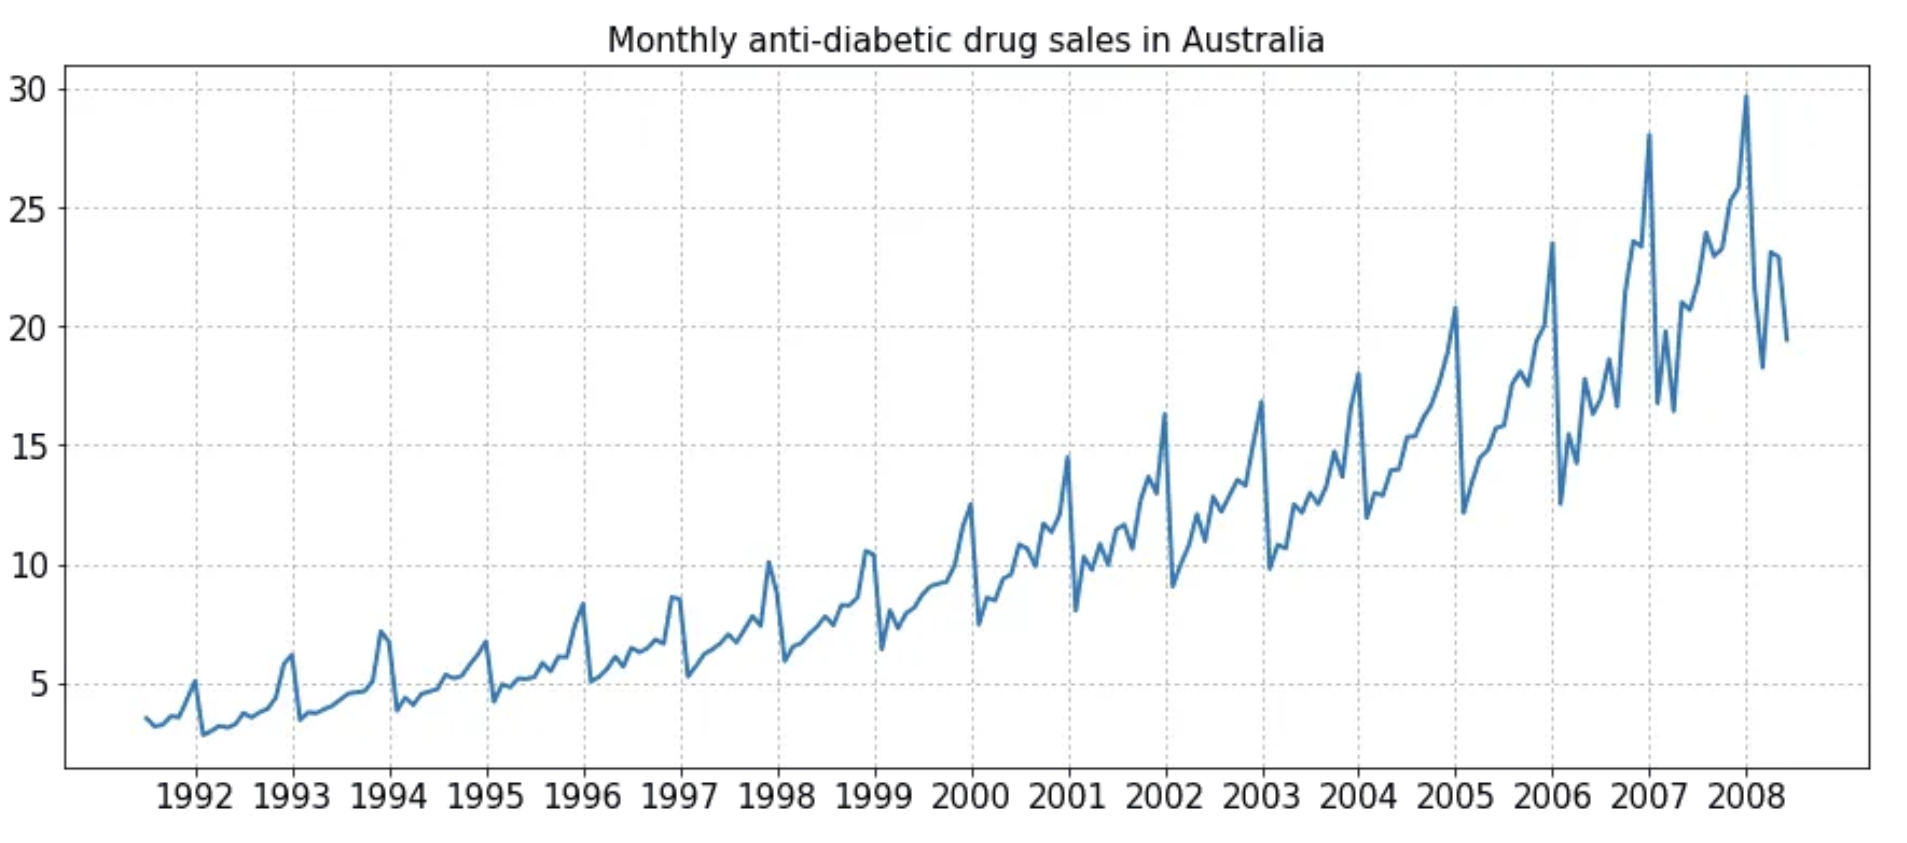
\includegraphics[width=0.7\textwidth]{trend_seasonality_example.png}
\end{frame}


\begin{frame}{Скользящее среднее}
\[
\tilde y_t=\frac{1}{k}\sum_{i=0}^{k-1} y_{t-i}
\]
\begin{itemize}
    \item Сглаживает шум и выделяет уровень ряда
    \item $k$ — длина окна недавней истории
    \item Малое $k$: быстрая реакция, больше шум
    \item Большое $k$: плавно, но с запаздыванием
\end{itemize}
\end{frame}


    \begin{frame}{Простое экспоненциальное сглаживание (SES)}
\[
\hat y_{t+1|t}
= \alpha y_t + (1-\alpha)\,\hat y_{t|t-1},
\qquad \alpha \in (0,1)
\]
\begin{itemize}
    \item Недавние значения имеют больший вес
    \item $\alpha$ — параметр памяти:
    \begin{itemize}
        \item $\alpha$ ближе к 1 → быстрые изменения, меньше сглаживание
        \item $\alpha$ ближе к 0 → сильное сглаживание, запаздывание
    \end{itemize}
    \item Для рядов без выраженного тренда
\end{itemize}
\end{frame}


\begin{frame}{Модель Холта: добавляем тренд}
\[
\ell_t=\alpha y_t + (1-\alpha)(\ell_{t-1}+b_{t-1})
\]
\[
b_t=\beta(\ell_t-\ell_{t-1}) + (1-\beta)b_{t-1}
\]
\[
\hat y_{t+h|t}=\ell_t + h\,b_t
\]
\begin{itemize}
    \item $\ell_t$ — оценка уровня ряда
    \item $b_t$ — оценка тренда (скорости изменения)
    \item $\alpha, \beta \in (0,1)$ — коэффициенты сглаживания
    \item Значения параметров подбирают по данным (минимизация ошибки прогноза)
\end{itemize}
\end{frame}


\begin{frame}{Хольта–Уинтерса: аддитивная сезонность}
\[
\ell_t=\alpha (y_t-s_{t-m}) + (1-\alpha)(\ell_{t-1}+b_{t-1})
\]
\[
b_t=\beta(\ell_t-\ell_{t-1}) + (1-\beta)b_{t-1}
\]
\[
s_t=\gamma (y_t-\ell_t) + (1-\gamma)s_{t-m}
\]
\[
\hat y_{t+h|t}=\ell_t + h\,b_t + s_{t+m_h}, \quad m_h=((h-1)\bmod m)+1
\]
\begin{itemize}
    \item $\ell_t$ — уровень, $b_t$ — тренд, $s_t$ — сезонность
    \item $\alpha, \beta, \gamma$ — коэффициенты сглаживания \((0,1)\)
    \item Сезонные колебания примерно одинаковой величины
\end{itemize}
\end{frame}


    \begin{frame}{Хольта–Уинтерса: мультипликативная сезонность}
\[
\ell_t=\alpha \frac{y_t}{s_{t-m}} + (1-\alpha)(\ell_{t-1}+b_{t-1})
\]
\[
b_t=\beta(\ell_t-\ell_{t-1}) + (1-\beta)b_{t-1}
\]
\[
s_t=\gamma \frac{y_t}{\ell_t} + (1-\gamma)s_{t-m}
\]
\[
\hat y_{t+h|t}=(\ell_t + h\,b_t)\,s_{t+m_h}
\]
\begin{itemize}
    \item Амплитуда сезонности растёт вместе с уровнем
    \item Используется для пропорциональных колебаний
\end{itemize}
\end{frame}


    \begin{frame}{Как выбрать модель сезонности?}
\begin{itemize}
    \item \textbf{Аддитивная}:
    \begin{itemize}
        \item сезонные колебания примерно постоянны по величине
    \end{itemize}
    \item \textbf{Мультипликативная}:
    \begin{itemize}
        \item амплитуда возрастает или уменьшается вместе с уровнем
    \end{itemize}
\end{itemize}
\centering
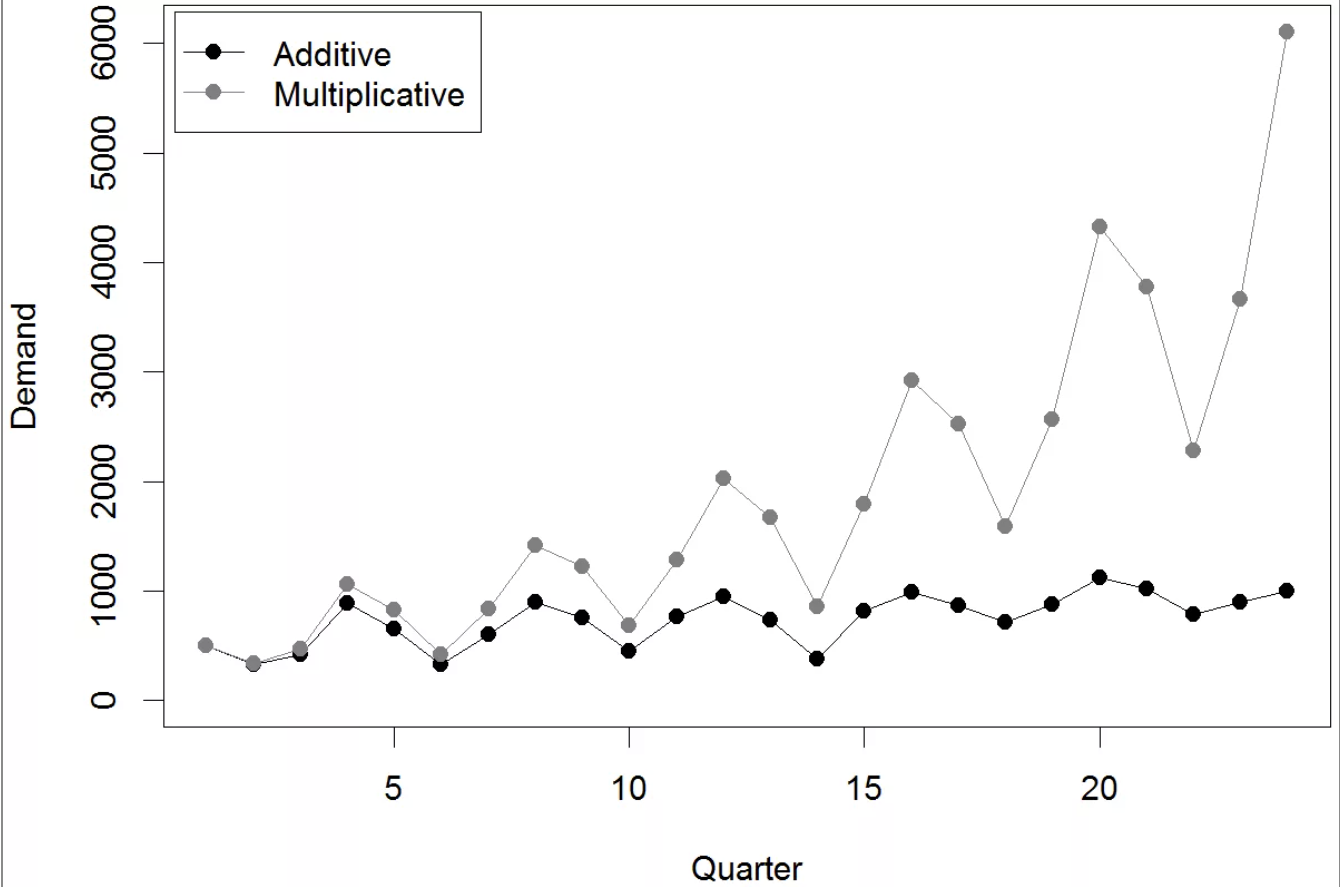
\includegraphics[width=0.6\textwidth]{additive_vs_multiplicative.png}
\end{frame}


% -------- БЛОК 3: Авторегрессионные модели --------

% 3.0 Введение
\begin{frame}{Авторегрессионные модели: идея и маршрут}
\begin{itemize}
  \item Цель: формально описать зависимость $y_t$ от прошлого и шумов
  \item База: лаги, ACF/PACF, стационарность и преобразования
  \item Семейства: AR, MA, ARMA, ARIMA; сезонные/расширенные: SARIMA, ARIMAX
\end{itemize}
\end{frame}

% 3.1 Лаги и лаговый оператор
\begin{frame}{Лаги и лаговый оператор}
\[
Ly_t = y_{t-1}, \qquad L^k y_t = y_{t-k}
\]
\[
(1-L)y_t = y_t - y_{t-1}, \qquad (1-L^m)y_t = y_t - y_{t-m}
\]
\begin{itemize}
  \item Лаг $\tau$ — сдвиг на $\tau$ шагов назад
  \item $(1-L)$ — обычная разность (убирает тренд), $(1-L^m)$ — сезонная разность с периодом $m$
\end{itemize}
\end{frame}

% 3.2 ACF и PACF
\begin{frame}{ACF и PACF: что смотреть перед моделированием}
\small
\[
r_\tau=\frac{\sum_{t=1}^{T-\tau}(y_t-\overline y)(y_{t+\tau}-\overline y)}{\sum_{t=1}^T (y_t-\overline y)^2},
\qquad
\overline y=\frac{1}{T}\sum_{t=1}^T y_t
\]
\begin{itemize}
  \item $r_\tau$ — автокорреляция на лаге $\tau$;\; $\overline y$ — среднее по выборке
  \item Пики на лагах $m,2m,\dots$ $\Rightarrow$ сезонность с периодом $m$
  \item Шаблоны: PACF «обрывается» для AR($p$);\; ACF «обрывается» для MA($q$)
\end{itemize}
\centering 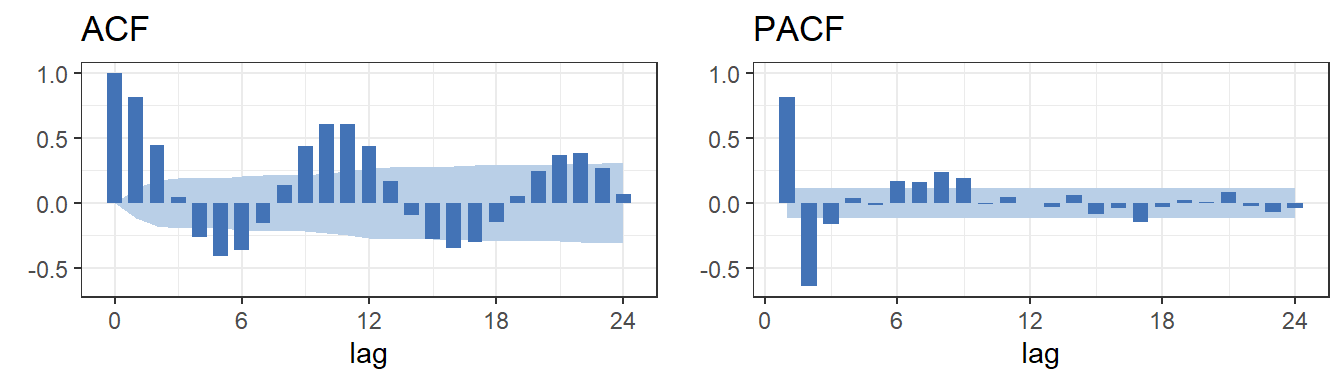
\includegraphics[width=0.72\textwidth]{acf_pacf_example.png}
\end{frame}

% 3.3 Стационарность: интуиция и два уровня
\begin{frame}{Стационарность: интуиция и два уровня}
\begin{itemize}
  \item Интуитивно: статистические свойства не меняются при сдвиге по времени
  \item \textbf{Узкий (строгий) смысл:} совместные распределения инвариантны к сдвигу
  \item \textbf{Широкий смысл:} $\mathbb{E}[y_t]=\mu$, $\mathrm{Var}(y_t)<\infty$,\\
  \hspace{1.15em}$\mathrm{cov}(y_{t+\tau},y_{s+\tau})=\mathrm{cov}(y_t,y_s)$ (зависит только от лага)
\end{itemize}
\end{frame}

% 3.4 Стационарность: пример и типичные нарушения
\begin{frame}{Стационарность: пример и типичные нарушения}
\small
\textbf{Пример (широкая, но не узкая):}\quad $y_t=\xi_1\cos t+\xi_2\sin t$, где $\xi_1,\xi_2\in\{\pm1\}$ независимы.\\
$\mathbb{E}[y_t]=0,\;\mathrm{cov}(y_t,y_s)=\cos(t-s)$, но распределения $y_0$ и $y_{\pi/4}$ различны.\\[0.45em]
\textbf{Типовые нарушения:}
\begin{itemize}
  \item \emph{Случайное блуждание:} $y_t=y_{t-1}+\varepsilon_t$ (дисперсия растёт)
  \item \emph{Линейный тренд:} $y_t=\alpha+\beta t+\varepsilon_t$ (среднее меняется)
  \item \emph{Чистая сезонность:} $y_t=\sin t+\varepsilon_t$ (среднее периодично)
\end{itemize}
\end{frame}

% 3.5 Приведение к стационарности
\begin{frame}{Приведение к стационарности: масштаб и разности}
\small
\[
z_t=
\begin{cases}
\dfrac{y_t^{\lambda}-1}{\lambda}, & \lambda\neq 0,\\[4pt]
\ln y_t, & \lambda=0
\end{cases}
\quad\text{— преобразование Бокса–Кокса}
\]
\[
(1-L)y_t=y_t-y_{t-1}, \qquad (1-L^m)y_t=y_t-y_{t-m}
\]
\begin{itemize}
  \item $\lambda$ — параметр Box–Cox; при $\lambda=0$ используется логарифм
  \item Практика: сначала $(1-L^m)$, затем при необходимости $(1-L)$ до приемлемой стационарности
\end{itemize}
\end{frame}

% 3.6 AR(p)
\begin{frame}{AR($p$): авторегрессия $p$-го порядка}
\[
y_t = \alpha + \phi_1 y_{t-1} + \dots + \phi_p y_{t-p} + \varepsilon_t
\]
\begin{itemize}
  \item $\varepsilon_t$ — белый шум (нуль-среднее, постоянная дисперсия, некоррелированность)
  \item AR(1): $y_t=\alpha+\phi y_{t-1}+\varepsilon_t$;\; если $|\phi|<1$, то стационарно;\; $r_h=\phi^h$
\end{itemize}
\end{frame}

% 3.7 MA(q)
\begin{frame}{MA($q$): скользящее среднее $q$-го порядка}
\[
y_t = \mu + \varepsilon_t + \theta_1 \varepsilon_{t-1} + \dots + \theta_q \varepsilon_{t-q}
\]
\begin{itemize}
  \item Память по прошлым возмущениям $\varepsilon_{t-i}$ — влияние постепенно затухает
  \item Параметры $\theta_i$ отражают силу и длительность «эхо» прошлых случайных колебаний
\end{itemize}
\end{frame}

% 3.8 ARMA(p,q)
\begin{frame}{ARMA($p,q$): объединяем AR и MA}
\[
y_t = \alpha + \phi_1 y_{t-1} + \dots + \phi_p y_{t-p}
      + \varepsilon_t + \theta_1 \varepsilon_{t-1} + \dots + \theta_q \varepsilon_{t-q}
\]
\[
a(L) y_t = \alpha + b(L)\varepsilon_t,\quad
a(L)=1-\phi_1L-\dots-\phi_p L^p,\;\; b(L)=1+\theta_1L+\dots+\theta_qL^q
\]
\end{frame}

% 3.9 ARIMA(p,d,q)
\begin{frame}{ARIMA($p,d,q$): работаем с нестационарностью}
\[
(1-L)^d y_t = y_t - y_{t-1}
\]
\[
a(L)(1-L)^d y_t = \alpha + b(L)\varepsilon_t
\]
\begin{itemize}
  \item $d$ — порядок дифференцирования (сколько раз берём разность) перед применением ARMA
\end{itemize}
\end{frame}

% 3.10 SARIMA
\begin{frame}{SARIMA: сезонная ARIMA}
\small
\[
\Phi(L^m)\,\phi(L)\,(1-L)^d(1-L^m)^D y_t = \Theta(L^m)\,\theta(L)\,\varepsilon_t + c
\]
\begin{itemize}
  \item $(p,d,q)$ — несезонные порядки; $(P,D,Q)_m$ — сезонные; $m$ — длина периода
  \item Учитываются краткосрочные лаги и сезонные лаги $m,2m,\dots$
\end{itemize}
\end{frame}

% 3.11 ARIMAX / SARIMAX
\begin{frame}{ARIMAX / SARIMAX: учитываем внешние факторы}
\[
(1-L)^d y_t = \mu + \sum_{i=1}^{n} \beta_i x_{t,i} + \frac{b(L)}{a(L)} \varepsilon_t
\]
\begin{itemize}
  \item $x_{t,i}$ — известные на момент прогноза факторы (например, календарь, температура)
  \item Внешние драйверы помогают снизить остаточную ошибку прогноза
\end{itemize}
\end{frame}

% 3.12 Итоги блока
\begin{frame}{Итоги блока: ARIMA-семейство}
\begin{itemize}
  \item \textbf{AR/MA/ARMA}: стационарные зависимости по лагах и шумам
  \item \textbf{ARIMA}: разности + ARMA для нестационарных рядов
  \item \textbf{SARIMA}: явная сезонность; \textbf{ARIMAX}: учёт известных факторов
\end{itemize}
\end{frame}

% ============================================
% БЛОК: RNN → LSTM → GRU (3 слайда)
% ============================================

% 1) Вводный слайд про RNN
\begin{frame}{От классики к RNN: идея рекуррентности}
\begin{itemize}
  \item В отличие от обычной (прямой) сети, рекуррентная сеть хранит \textbf{скрытое состояние} $h_t$
  \item На каждом шаге учитываются и \textbf{текущий вход} $x_t$, и \textbf{память} $h_{t-1}$
  \item Типичная запись: \;$h_t=\tanh(W_{xh}x_t+W_{hh}h_{t-1}+b_h)$,\quad $\hat y_t=g(W_{hy}h_t+b_y)$
  \item \textbf{Проблема:} при длинных последовательностях градиент \textit{затухает/взрывается} \,$\Rightarrow$ новая информация слабо влияет
\end{itemize}
\end{frame}

% 2) Коротко про LSTM
\begin{frame}{LSTM: как стабилизировать память на длинных шагах}
\begin{columns}[T,onlytextwidth]
\column{0.55\textwidth}
\begin{itemize}
  \item Идея: \textbf{вентили} управляют потоком информации
  \item Компоненты: забывание $f_t$, вход $i_t$, выход $o_t$, состояние ячейки $C_t$
  \item Ключевая «магистраль» памяти:
  \[
  C_t = f_t \odot C_{t-1} + i_t \odot \tilde{C}_t
  \]
  \item Эффект: градиент течёт по почти линейному пути через $C_t$ $\Rightarrow$ меньше затухания/взрыва
\end{itemize}
\footnotesize
\textit{Детали пропускаем: коллега уже разбирал математику LSTM на прошлом докладе.}
\column{0.42\textwidth}
\centering
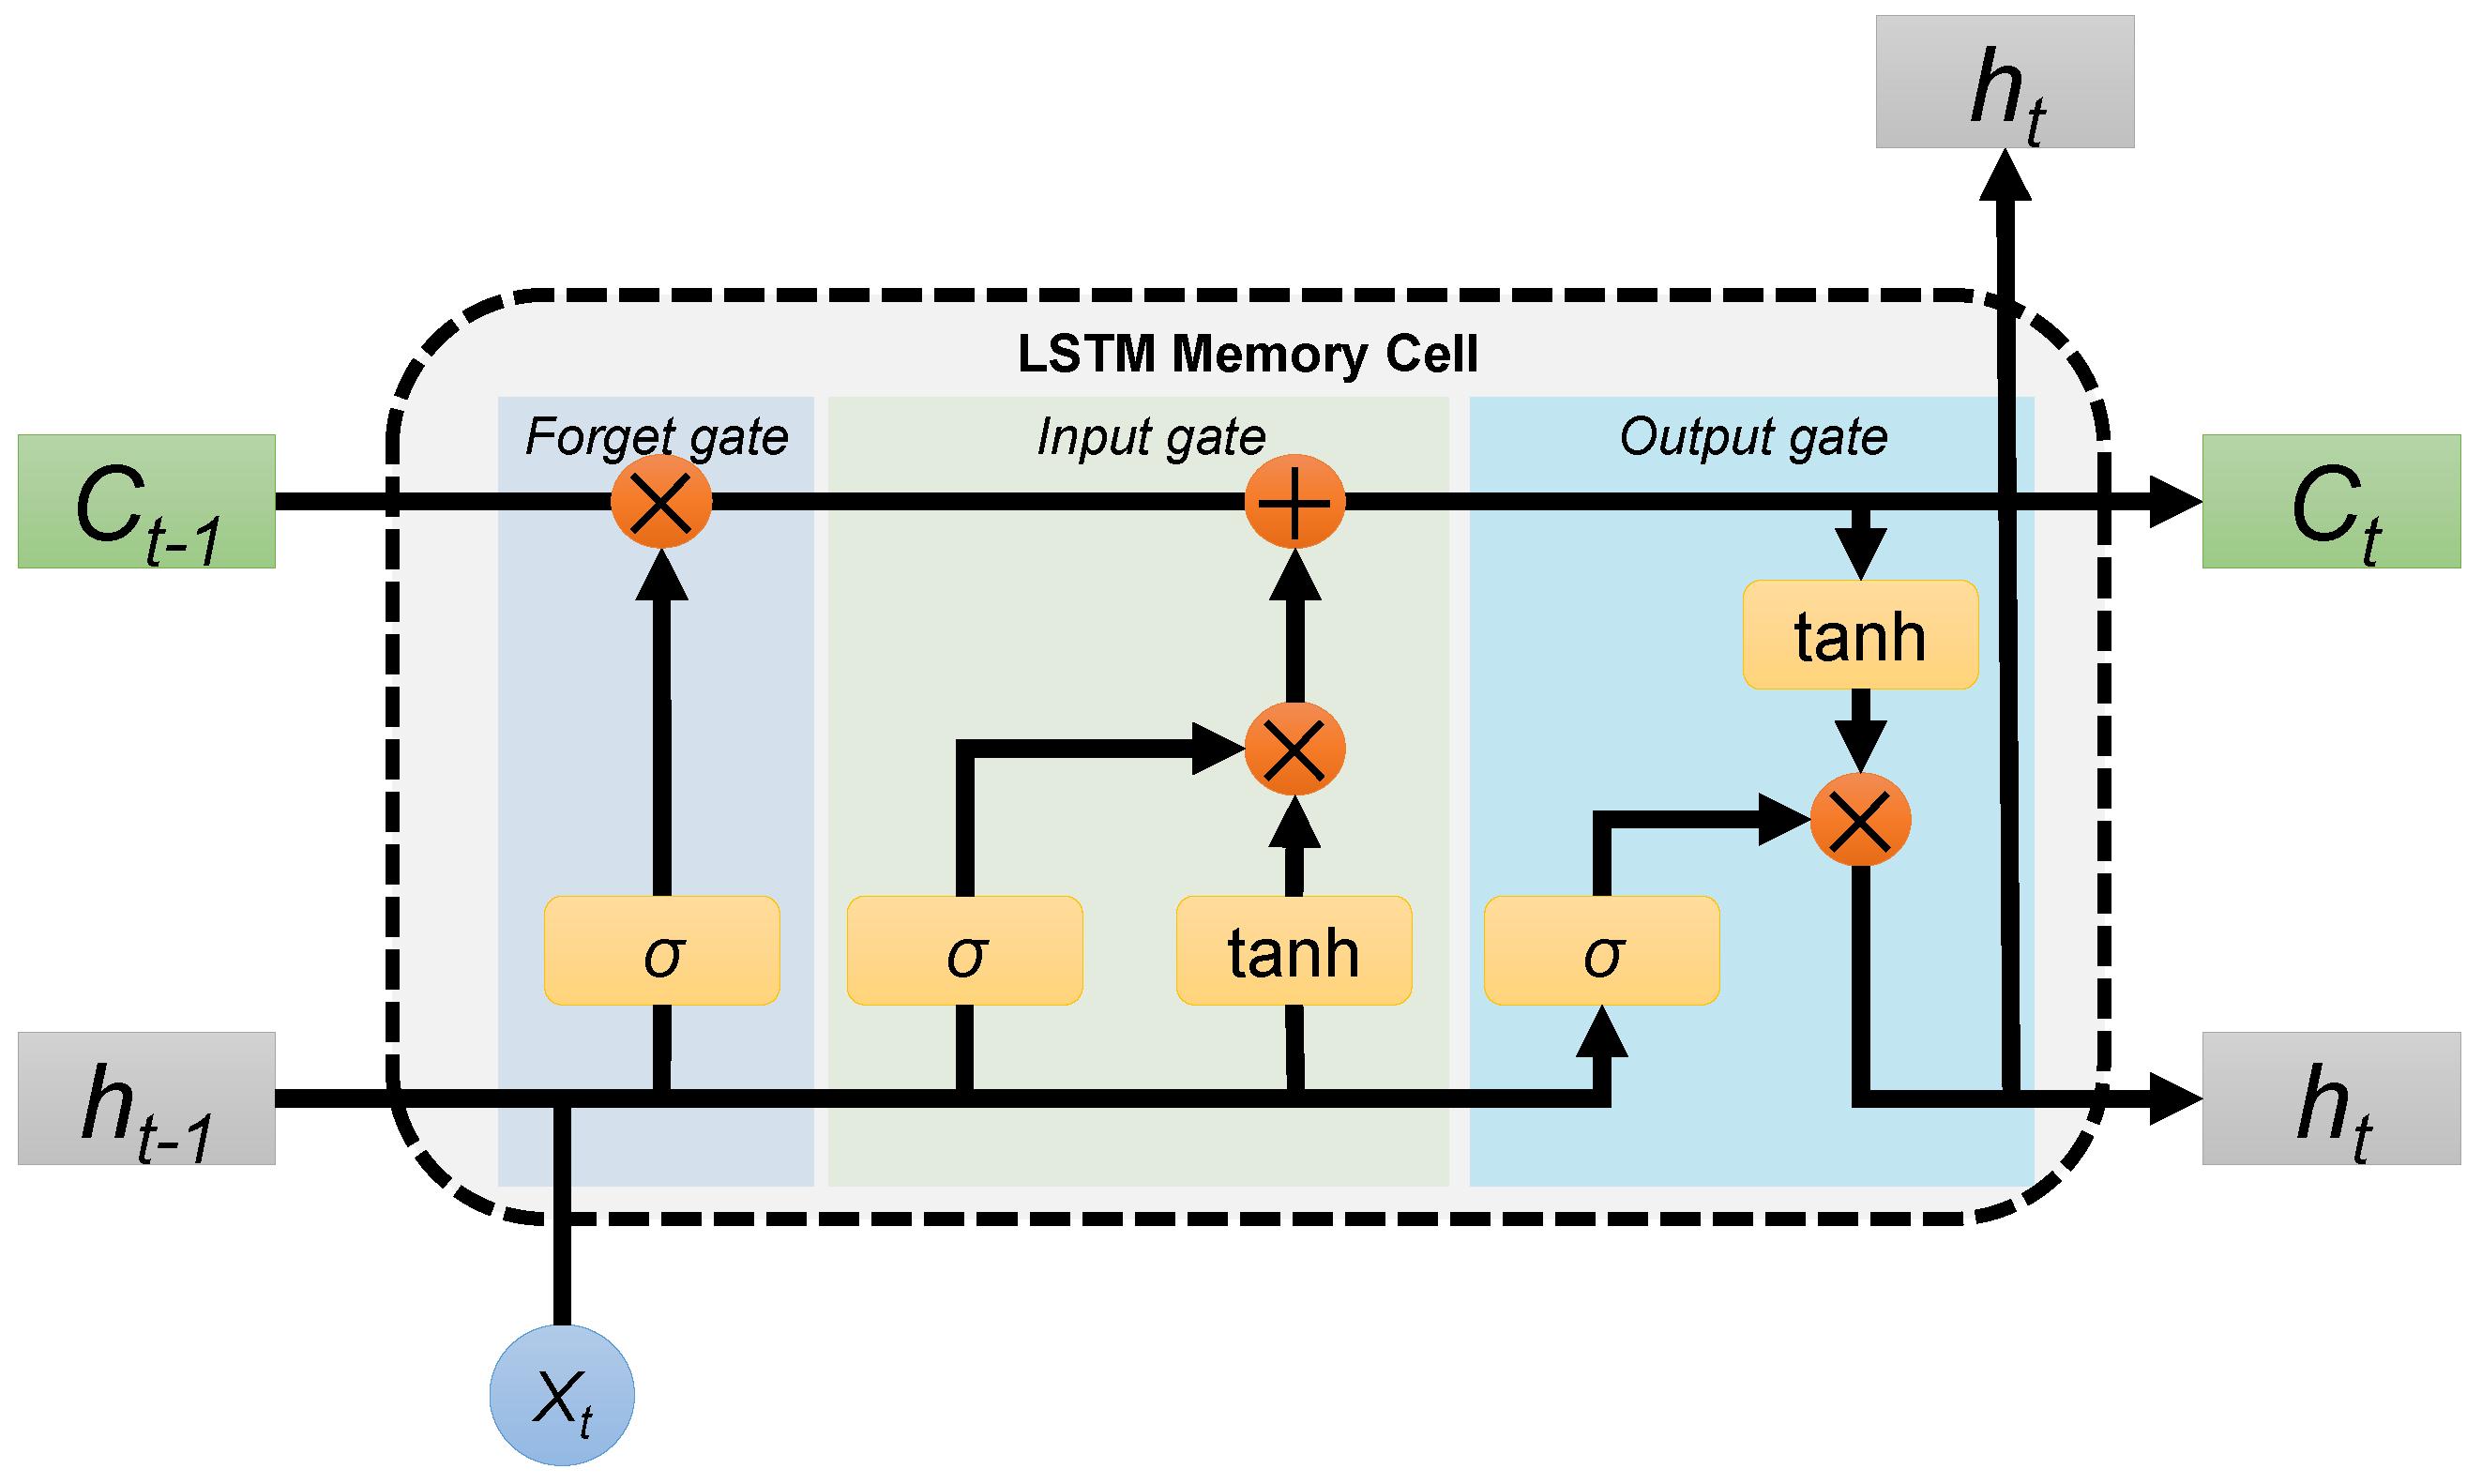
\includegraphics[width=\linewidth]{LSTM.png}\\
\footnotesize Схема LSTM-ячейки
\end{columns}
\end{frame}

% 3) GRU с формулами и порядком вычислений
\begin{frame}{GRU: упрощённая альтернатива LSTM (порядок вычислений)}
\small
\[
\begin{aligned}
\textbf{(1) Вентиль обновления:}\quad
& z_t = \sigma(W_z x_t + U_z h_{t-1} + b_z) \\
\textbf{(2) Вентиль сброса:}\quad
& r_t = \sigma(W_r x_t + U_r h_{t-1} + b_r) \\
\textbf{(3) Кандидат состояния:}\quad
& \tilde{h}_t = \tanh\!\big(W_h x_t + U_h (r_t \odot h_{t-1}) + b_h\big) \\
\textbf{(4) Обновление памяти:}\quad
& h_t = (1 - z_t)\odot h_{t-1} + z_t \odot \tilde{h}_t
\end{aligned}
\]
\begin{itemize}
  \item Нет отдельного $C_t$: память и выход объединены в $h_t$
  \item \textbf{Хронология шага $t$:} сначала $z_t, r_t$ $\rightarrow$ затем $\tilde{h}_t$ $\rightarrow$ затем $h_t$
  \item Интуиция: $r_t$ дозирует влияние прошлого в кандидате, $z_t$ решает, \emph{насколько} обновлять состояние
\end{itemize}
\end{frame}


% ============================================
% БЛОК: Attention — введение и мотивация
% ============================================

\begin{frame}{От RNN к Attention: обработка и генерация последовательностей}
\begin{itemize}
  \item Рекуррентные сети хорошо моделируют временные зависимости, но выдают выход фиксированной длины.
  \item Во многих задачах нужно предсказывать \textbf{последовательности произвольной длины} — например, в машинном переводе, где длина перевода не совпадает с длиной исходной фразы.
  \item Возникает архитектура \textbf{Sequence-to-Sequence (Seq2Seq)}:
  \begin{itemize}
    \item \textbf{Энкодер} считывает входную последовательность и преобразует её в векторное представление — «контекст».
    \item \textbf{Декодер} шаг за шагом генерирует выходную последовательность, опираясь на этот контекст.
  \end{itemize}
  \item Проблема: один фиксированный вектор не способен вместить всю информацию о длинной последовательности.
  \item Решение — \textbf{механизм внимания (Attention)}, который позволяет декодеру выбирать, на какие части входа смотреть в каждый момент.
\end{itemize}
\end{frame}


% ============================================
% БЛОК: Attention — механизм внимания
% ============================================

\begin{frame}{Механизм внимания (Attention)}
\small
\textbf{Идея:} на каждом шаге декодер сам решает, \emph{на какие части входа смотреть}, формируя индивидуальный контекст.

\begin{itemize}
  \item Пусть энкодер выдал скрытые состояния: $H = (h_1, \dots, h_T)$
  \item На $i$-м шаге декодер имеет своё состояние $s_i$
  \item Сравниваем $s_i$ с каждым $h_j$ и считаем \textbf{оценки внимания}:
  \[
  e_{i,j} = \mathrm{score}(s_i, h_j)
  \]
  \item Считаем веса через softmax:
  \[
  \alpha_{i,j} = \frac{\exp(e_{i,j})}{\sum_k \exp(e_{i,k})}
  \]
  \end{itemize}
\end{frame}

\begin{frame}{Механизм внимания (Attention)}
\begin{itemize}
  \item Формируем \textbf{контекстный вектор} — взвешенную сумму по входным состояниям:
  \[
  a_i = \sum_{j=1}^T \alpha_{i,j} h_j
  \]
  \item Контекст $a_i$ используется декодером для генерации очередного токена $y_i$
\end{itemize}

\footnotesize
\vspace{0.3em}
\textbf{Интерпретация:} $\alpha_{i,j}$ показывает, насколько важна позиция $j$ входа при генерации $i$-го выхода.
Механизм внимания снимает ограничение на один фиксированный контекст и даёт модели возможность
динамически фокусироваться на релевантных фрагментах входной последовательности.
\end{frame}

% ============================================
% БЛОК: Self-Attention (часть 1)
% ============================================

\begin{frame}{Self-Attention: идея и формирование Q, K, V}
\small
\textbf{Мотивация.}
Классический механизм внимания связывает энкодер и декодер,
но внутри одной последовательности токены тоже зависят друг от друга.
\textbf{Self-Attention} позволяет каждому токену смотреть на другие токены
в том же предложении и формировать контекст, учитывающий всю последовательность.

\vspace{0.4em}
\textbf{1. Вход.}
Пусть есть предложение: «кошка сидит на столе».
Каждый токен преобразуется в embedding $x_i \in \mathbb{R}^d$.
Все векторы объединяются в матрицу:
\[
X = [x_0, x_1, \dots, x_n] \in \mathbb{R}^{(n+1)\times d}.
\]

\vspace{0.4em}
\textbf{2. Формируем три набора векторов: Queries, Keys, Values.}
\[
Q_i = x_i W_Q, \quad K_i = x_i W_K, \quad V_i = x_i W_V,
\]
где $W_Q, W_K, W_V \in \mathbb{R}^{d\times d}$ — обучаемые матрицы.
\end{frame}



\begin{frame}{Self-Attention: вычисление внимания и контекста}
\small
\textbf{Интерпретация:}
\begin{itemize}
  \item $Q$ — «от кого идёт внимание» (что ищет токен),
  \item $K$ — «на кого направлено внимание»,
  \item $V$ — «какая информация передаётся».
\end{itemize}
На этом этапе каждый токен получает три разные роли, хотя исходный embedding был один.




\textbf{3. Вычисляем оценки внимания (scores).}
Для токена $i$ сравниваем его $Q_i$ со всеми $K_j$:
\[
\text{score}_{ij} = Q_i \cdot K_j.
\]
Так получаем вектор оценок — насколько каждый токен $j$ важен для токена $i$.

\vspace{0.4em}
\textbf{4. Преобразуем оценки в веса.}
\[
\alpha_{ij} = \mathrm{softmax}(\text{score}_{ij})
\]
Теперь для токена $i$ мы знаем, с какой важностью учитывать каждый другой токен.
\end{frame}
\begin{frame}{Self-Attention: вычисление внимания и контекста}
\small
\vspace{0.4em}
\textbf{4. Преобразуем оценки в веса.}
\[
\alpha_{ij} = \mathrm{softmax}(\text{score}_{ij})
\]
Теперь для токена $i$ мы знаем, с какой важностью учитывать каждый другой токен.
\vspace{0.4em}
\textbf{5. Формируем контекстный вектор.}
\[
\text{output}_i = \sum_j \alpha_{ij} V_j
\]
Каждый выход $output_i$ — это новый embedding токена $i$, который уже учитывает весь контекст предложения.

\end{frame}

\begin{frame}{Маскирование (Masking)}
\small
\textbf{Зачем:}
в авторегрессионных задачах модель не должна смотреть в будущее.

\vspace{0.4em}
\textbf{Причинная маска:}
\[
M_{ij} =
\begin{cases}
0, & j \le i,\\
-\infty, & j > i,
\end{cases}
\qquad
A = \mathrm{softmax}\!\left(\frac{QK^\top}{\sqrt{d_k}} + M\right)
\]

\vspace{0.4em}
Элементы $-\infty$ зануляются после softmax —
модель видит только прошлые токены.
\end{frame}

% ---------- БЛОК: Transformer ----------
\begin{frame}{Transformer: обзор архитектуры}
\begin{columns}[T,onlytextwidth]
\column{0.58\textwidth}
\begin{itemize}
  \item Без RNN/конв: полностью на механизме внимания — позволяет параллельно обрабатывать всю последовательность.
  \item Базовые блоки: Multi-Head Self-Attention, Add\&Norm, позиционные кодировки, Position-wise FFN.
  \item Encoder / Decoder — оба состоят из повторяющихся слоёв этих блоков.
\end{itemize}
\column{0.42\textwidth}
\centering
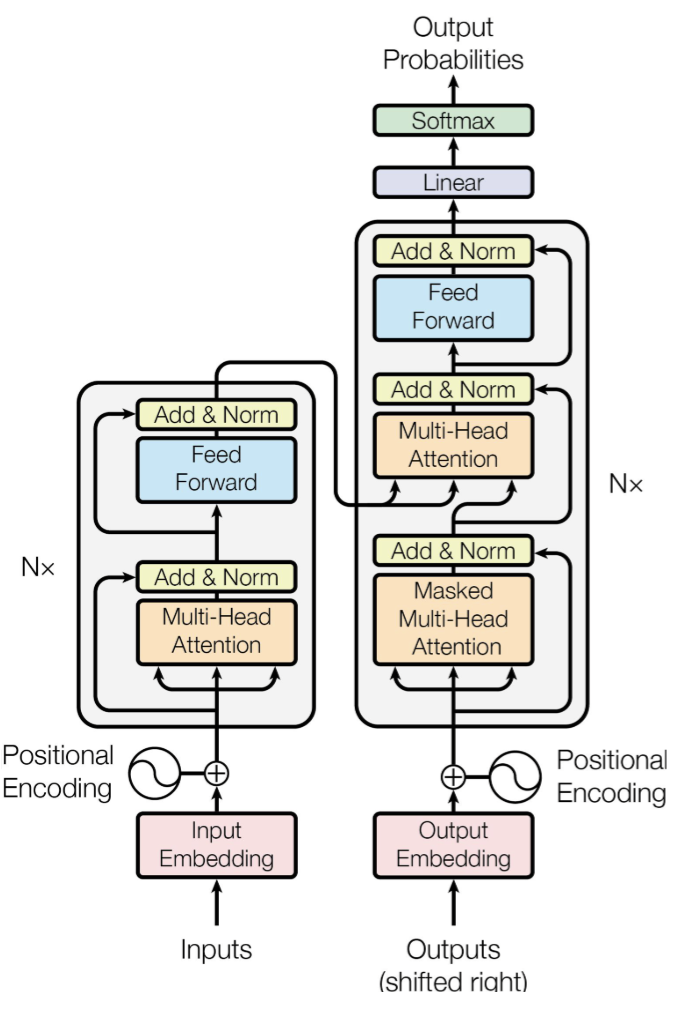
\includegraphics[width=\linewidth]{transformer.png}\\
\footnotesize Схема архитектуры Transformer (вход → энкодер → декодер → выход)
\end{columns}
\end{frame}

\begin{frame}{Scaled dot-product attention (формула и смысл)}
\small
Пусть для набора позиций заданы матрицы запросов, ключей и значений $Q, K, V$ ($Q,K \in \mathbb{R}^{n\times d_k},\; V\in\mathbb{R}^{n\times d_v}$). Тогда:
\[
\mathrm{Attention}(Q,K,V)=\mathrm{softmax}\!\left(\frac{QK^\top}{\sqrt{d_k}}\right)V.
\]
\begin{itemize}
  \item $QK^\top$ — попарные скоры между запросами и ключами.
  \item Деление на $\sqrt{d_k}$ стабилизирует распределение скоров при больших размерностях.
  \item softmax даёт веса внимания по каждой позиции; итог — взвешенная сумма по значениям $V$.
\end{itemize}
\end{frame}

\begin{frame}{Multi-Head self-attention (формулы и мотивация)}
\small
\[
\text{head}_i = \mathrm{Attention}(QW_i^Q,\;KW_i^K,\;VW_i^V),\qquad
\mathrm{MultiHead}(Q,K,V) = \mathrm{Concat}(\text{head}_1,\dots,\text{head}_h)W^O.
\]
\begin{itemize}
  \item Каждая голова — собственное линейное проецирование Q/K/V → разные «взгляды» на зависимости.
  \item Конкатенация + выходная проекция объединяют информацию от всех голов.
  \item Self-attention = Q,K,V берутся из одного и того же слоя (токен обращается к другим токенам в той же последовательности).
\end{itemize}
\end{frame}

\begin{frame}{Позиционные кодировки (почему и как)}
\small
\begin{itemize}
  \item Attention сам по себе не учитывает порядок — нужна информация о позиции токена.
  \item Оригинальный вариант (синусно-косинусные):
\end{itemize}
\[
\begin{aligned}
\mathrm{PE}_{pos,2i} &= \sin\!\left(\frac{pos}{10000^{2i/d_\text{model}}}\right),\\
\mathrm{PE}_{pos,2i+1} &= \cos\!\left(\frac{pos}{10000^{2i/d_\text{model}}}\right).
\end{aligned}
\]
\begin{itemize}
  \item Такие кодировки дают постоянные периодические шаблоны, позволяющие моделям аппроксимировать относительный порядок и сдвиги.
  \item Альтернативы: обучаемые позиционные эмбеддинги, относительные позиционные кодировки.
\end{itemize}
\end{frame}

\begin{frame}{Position-wise Feed-Forward Network (FFN)}
\small
После слоя внимания каждый токен проходит независимую небольшую MLP:
\[
\mathrm{FFN}(x) = \mathrm{Activation}(xW_1 + b_1)W_2 + b_2,
\]
где обычно \(\mathrm{Activation}=\mathrm{ReLU}\) или \(\mathrm{GELU}\).
\begin{itemize}
  \item FFN применяется отдельно к каждому положению (position-wise), не смешивая информацию между токенами — это даёт нелинейную проекцию признаков.
  \item Типичный выбор: увеличение размерности в скрытом слое (например, $d_\text{model}\to 4d_\text{model}\to d_\text{model}$).
\end{itemize}
\end{frame}

\begin{frame}{Add \& Norm (Residual + LayerNorm)}
\small
В каждом субблоке используется остаточное соединение и нормализация:
\[
\text{SublayerOutput} = \mathrm{LayerNorm}(x + \text{Sublayer}(x)).
\]
\begin{itemize}
  \item Residual (skip) соединение ускоряет оптимизацию и помогает градиенту проходить через глубокие слои.
  \item LayerNorm нормализует по признакам каждого токена независимо (по feature-dimension).
  \item Нормализация делается по токену, а не по батчу — это критично для NLP (см. следующую страницу).
\end{itemize}
\end{frame}

\begin{frame}{Почему LayerNorm, а не BatchNorm? (важно)}
\small
\begin{itemize}
  \item В трансформерах нормализуем \textbf{каждый токен отдельно по признакам}, а не по всем токенам или батчу.
  \item Причины:
  \begin{itemize}
    \item Разная длина последовательностей: нормализация по всем токенам или батчу потребовала бы учитывать паддинги, искажая статистику.
    \item Семантика токенов различна: токены — слова/части слов, их значения несопоставимы, поэтому «сквозная» нормализация между токенами бессмысленна.
    \item Стабильность при inference: генерация авторегрессивно идёт по одному токену; LayerNorm не зависит от других токенов → одинаковое поведение при обучении и при генерации.
    \item Независимость от батча: BatchNorm требует статистику по батчу; в NLP батчи часто малы и разношироки → статистика шумная. LayerNorm работает корректно даже при batch_size=1.
  \end{itemize}
\end{itemize}
\end{frame}

\begin{frame}{Короткое резюме: роль компонентов Transformer}
\begin{itemize}
  \item Self-attention — гибкий механизм для установления длинно- и коротко- диапазонных зависимостей, полностью параллельный.
  \item Multi-head — разные представления/внимания в параллели.
  \item Позиционные кодировки — вводят порядок в безпорядочную матрицу внимания.
  \item FFN — проекция на позицию для внесения нелинейности и увеличения выразительности.
  \item Add\&Norm (Residual + LayerNorm) — стабилизация обучения и согласованное поведение при inference.
\end{itemize}
\end{frame}

\begin{frame}{Заключение}
\begin{itemize}
    \item Прогнозирование временных рядов прошло длинный путь:
    от интерпретируемых статистических моделей (ARIMA, ETS)
    к мощным нейросетевым архитектурам (LSTM, Transformer).
    \item Классические подходы хорошо работают при ограниченных данных,
    чёткой сезонности и трендах.
    \item Нейросетевые методы раскрывают потенциал при больших объёмах данных
    и сложных нелинейных зависимостях.
    \item Современные трансформеры объединяют гибкость self-attention
    и параллельность обучения, становясь универсальным инструментом
    для анализа последовательностей — от текста до временных рядов.
    \item Направления развития: гибридные модели (ARIMA+NN),
    энергоэффективные архитектуры и использование контекстных признаков.
\end{itemize}
\vspace{0.6em}
\centering
\textbf{Главная идея:} модели усложняются, но цель остаётся прежней —\\
\textit{научиться понимать и предсказывать динамику процессов во времени.}
\end{frame}


\end{document}
